\begin{frame}{Lenguajes de Programación}
\justifying
Es una forma de comunicarse con el ordenador, principalmente son de tres niveles:

\begin{itemize}
\item Alto nivel
\item Bajo nivel
\item Lenguaje máquina
\end{itemize}

En nuestro caso utilizaremos \textbf{Python} y este es de alto nivel.
\end{frame}

\begin{frame}{Tipos de lenguajes de Programación}
\justifying
Hay lenguajes de tipo compilado e interpretado, y Python es interpretado, de esto nos damos cuenta cuando se observa la ejecución de los scripts en consola sin la necesidad de crear un nuevo archivo.

\begin{figure}[H]
\centering
\includegraphics[scale=0.2]{Section_Files/images/chapter01/01.png}
\end{figure}
\end{frame}